\chapter{Diseño e implementación}
\label{cap:DisenioImplementacion}

En este capítulo se presenta la arquitectura de hardware y software del dispositivo de captura, como así también del generador de señal MVB desarrollado para probar el dispositivo de captura sin necesidad de conectarlo en una formación ferroviaria.

\section{Arquitectura de hardware}
\label{sec:hardware}

Como se muestra en la figura~\ref{fig:conexion}, el dispositivo de captura tiene dos conectores DE-9 compatibles con el medio EMD. De esta manera se lo puede conectar a un segmento MVB entre dos dispositivos cualesquiera.

\begin{figure}[htbp]
	\centering
    {
        \fontfamily{phv}
        \fontsize{8pt}{8pt}\selectfont
        \input{./Figures/conexion.pdf_tex}
    }
	\caption{Conexión del dispositivo de captura en un segmento EMD.}
    \label{fig:conexion}
\end{figure}

En la figura~\ref{fig:bloques} se muestra un diagrama de la arquitectura del dispositivo de captura.
Se dejan en corto circuito las líneas de transmisión (ver figura~\ref{fig:pines}), de forma tal de que el dispositivo opere en forma pasiva. Salvando la impedancia que agrega a la línea, el dispositivo de captura es transparente para el resto de los dispositivos del segmento.
El dispositivo MAX485 \cite{max485} se utiliza para convertir la señal de entrada (par diferencial $-$5~V - +5~V) a una señal compatible para el analizador lógico VKTECH (0~V - +5~V). El analizador lógico se conecta a una Raspberry Pi mediante un puerto USB 2.0. La Raspberry Pi decodifica las tramas por software y almacena los datos capturados en una tarjeta de memoria. Mediante su interfaz Wi-Fi se puede conectar una PC (utilizando el protocolo SSH) para descargar las capturas, y también para visualizar el tráfico del bus MVB en tiempo real.

\begin{figure}[htbp]
	\centering
    {
        \fontfamily{phv}
        \fontsize{8pt}{8pt}\selectfont
        \input{./Figures/bloques.pdf_tex}
    }
	\caption{Arquitectura de hardware del dispositivo de captura.}
    \label{fig:bloques}
\end{figure}

En la figura~\ref{fig:esquematico} se muestra un diagrama esquemático con el detalle de las conexiones entre los diferentes componentes. En el diagrama se utiliza la etiqueta ``USB'' para representar la conexión a la Raspberry Pi, que no se muestra por simplicidad. Asimismo, la conexión ``VCC'' del MAX485 se conecta al pin número 2 del conector GPIO de la Raspberry Pi \cite{gpio}.

\begin{figure}[htbp]
	\centering
	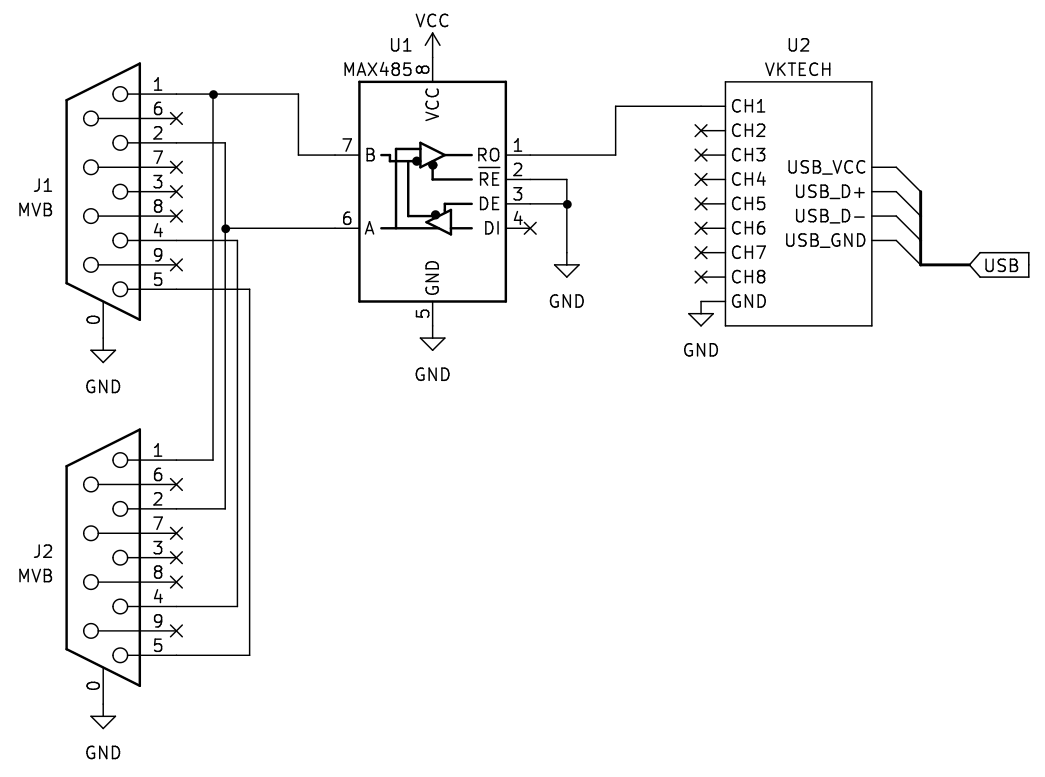
\includegraphics[width=1\textwidth]{./Figures/esquematico.png}
	\caption{Diagrama esquemático del dispositivo de captura.}
    \label{fig:esquematico}
\end{figure}

En la figura~\ref{fig:fotodispositivo} se muestra una foto del dispositivo de captura en construcción. Cabe aclarar que en el dispositivo hay cuatro MAX485 para permitir, en el futuro, capturar ambas líneas A y B del segmento EMD, o bien capturar dos o más segmentos diferentes. En esta primera versión del dispositivo se utiliza solo uno de los MAX485.

\begin{figure}[htbp]
	\centering
	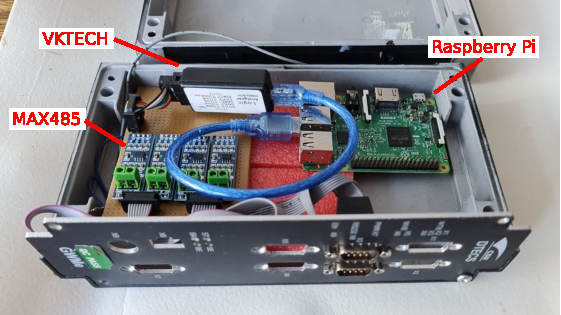
\includegraphics[width=1\textwidth]{./Figures/foto-dispositivo.pdf}
	\caption{Foto del dispositivo de captura en construcción.}
    \label{fig:fotodispositivo}
\end{figure}

\section{Arquitectura de software}
\label{sec:software}

Como se ve en la figura~\ref{fig:bloques}, la señal digital capturada por el VKTECH se envía a la Raspberry Pi en tiempo real mediante la interfaz USB. Para recibir esta señal en la Raspberry Pi se utiliza Sigrok, invocándolo de la siguiente manera:

\begin{lstlisting}
sigrok-cli -d fx2lafw --continuous --config samplerate=12m
           --channels D0 -O binary
\end{lstlisting}

Los parámetros utilizados son:

\begin{itemize}
        \item \texttt{-d fx2lafw}: Utilizar el \textit{driver} compatible con el dispositivo VKTECH.
        \item \texttt{--continuous}: Muestrear en forma continua hasta ser detenido.
        \item \texttt{--config samplerate=12m}: Muestrear con una frecuencia de 12 MHz.
        \item \texttt{--channels D0}: Muestrear únicamente el canal 0 (correspondiente al pin \texttt{CH1} de la figura \ref{fig:esquematico}).
        \item \texttt{-O binary}: Producir como salida un flujo de datos en formato binario.
\end{itemize}

Por cada muestra capturada, se emite un byte en el que cada bit corresponde a uno de los 8 canales del VKTECH.
Como se captura únicamente el canal 0, el bit menos significativo será 0 o 1 dependiendo de si la señal lógica capturada es baja o alta.
De esta forma, el flujo de datos tiene un ancho de banda de 12 MB/s, aunque se usa solo uno de los 8 bits de cada byte.
Este flujo de datos se puede redireccionar a un archivo o a un \textit{pipe} de Unix.

En la figura~\ref{fig:sigrok} se muestra un ejemplo del flujo de datos producido por Sigrok. El intervalo de 666,7 ns corresponde a un bit de datos de una trama MVB en codificación Manchester (ver figura~\ref{fig:manchester}). La frecuencia de muestreo de 12 MHz produce una muestra cada 83,33 ns.

\begin{figure}[htbp]
	\centering
    {
        \fontfamily{phv}
        \fontsize{9pt}{9pt}\selectfont
        \input{./Figures/sigrok.pdf_tex}
    }
	\caption{Flujo de datos producido por Sigrok.}
    \label{fig:sigrok}
\end{figure}

Sería posible bajar la frecuencia de muestreo, pero dado que la señal MVB se transmite a 1,5 Mbit/s en codificación Manchester, para lograr una captura suficientemente confiable el límite inferior es 6 MHz.
Sin embargo, la captura en una frecuencia cercana al límite inferior aumenta considerablemente la tasa de errores de captura.
La frecuencia elegida de 12 MHz ofrece un buen balance entre confiabilidad y eficiencia en espacio.

El flujo de datos producido por Sigrok se redirecciona mediante un \textit{pipe} de Unix a un software programado en lenguaje Go. Como se muestra en la figura~\ref{fig:capas-software}, la decodificación se realiza en tres capas de procesamiento:

\begin{enumerate}
\item La capa inferior (\texttt{MVBStream}) lee el flujo de datos byte por byte y ofrece funcionalidades tales como leer muestras individualmente, esperar hasta la siguiente transición de estado (alto-bajo o bajo-alto), esperar una cantidad de tiempo, etc.
\item La capa intermedia (\texttt{MVBDecoder}) identifica las tramas MVB y por cada telegrama produce un evento (\texttt{Event}).
\item La capa superior recibe los eventos y los procesa según el modo de operación del software. Se ofrecen dos modos de operación:
    \begin{itemize}
        \item En el modo interactivo, el software presenta una interfaz de usuario en la que se muestra el tráfico MVB en tiempo real. En la figura~\ref{fig:interactivo} se muestra una captura de pantalla del modo interactivo.
        \item En el modo de almacenamiento, el software permite almacenar la evolución histórica de una o más variables de importancia.
    \end{itemize}
\end{enumerate}

\begin{figure}[htbp]
	\centering
    {
        \fontfamily{phv}
        \fontsize{9pt}{9pt}\selectfont
        \input{./Figures/capas-software.pdf_tex}
    }
	\caption{Capas de procesamiento del software de captura.}
    \label{fig:capas-software}
\end{figure}

\begin{figure}[htbp]
	\centering
	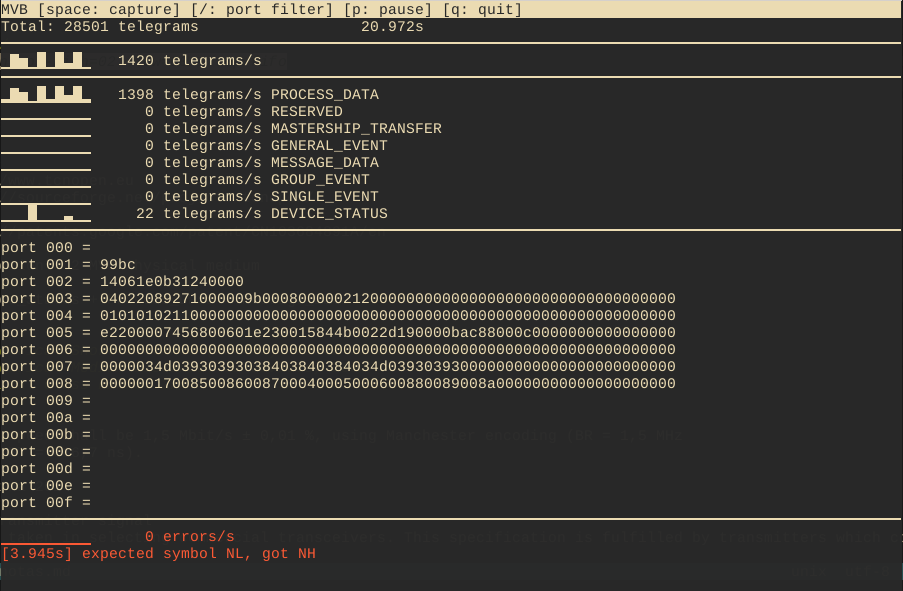
\includegraphics[width=1\textwidth]{./Figures/modo-interactivo.png}
	\caption{Modo interactivo del software de captura.}
    \label{fig:interactivo}
\end{figure}

El código fuente de este programa está disponible en la plataforma Github \cite{mvbparse-go}.
En el archivo \texttt{README.md} se muestran más detalles acerca de los diferentes modos de funcionamiento.

\section{Dispositivo generador de señal}
\label{sec:generador}
